\documentclass[12pt,a4paper]{article}

% ── Packages ─────────────────────────────────────────────────────────────────
\usepackage[margin=2.5cm]{geometry}
\usepackage{amsmath,amssymb}
\usepackage{graphicx}
\usepackage{subcaption}
\usepackage{booktabs}
\usepackage{hyperref}
\usepackage{cite}
\usepackage{float}
\usepackage{lineno}
\usepackage{setspace}
\usepackage{xcolor}
\usepackage{listings}
\usepackage{authblk}
\usepackage{abstract}

% ── Code listing style ────────────────────────────────────────────────────────
\lstset{
  language=Python,
  basicstyle=\footnotesize\ttfamily,
  keywordstyle=\color{blue},
  commentstyle=\color{gray},
  stringstyle=\color{red!70!black},
  numbers=left, numberstyle=\tiny\color{gray},
  breaklines=true, frame=single,
  columns=fullflexible
}

\hypersetup{colorlinks=true, linkcolor=blue, citecolor=blue, urlcolor=blue}

% ── Title block ───────────────────────────────────────────────────────────────
\title{\Large\textbf{Self-Organized Criticality in Forest Fire Dynamics:\\
A Computational Study of the Drossel--Schwabl Model}}

\author{Submitted By: 2021CH70455, Siddhant Sudhakar Dhirde}
\date{Date of submission: April 10, 2026}

% ─────────────────────────────────────────────────────────────────────────────
\begin{document}
\maketitle
\begin{abstract}
\noindent
Self-organized criticality (SOC) is a universal mechanism through which many
dissipative systems spontaneously evolve toward a critical state without
external fine-tuning, giving rise to scale-free behaviour characterised by
power-law statistics. This paper investigates SOC in a forest fire system
using the Drossel--Schwabl cellular automaton (CA) model. A stochastic CA is
implemented on a $128\times128$ lattice with two connectivity topologies
(4-neighbour and 8-neighbour) at a growth-to-lightning ratio $p/f = 100$.
Following a burn-in of 2\,000 steps, over 10\,000 fire-avalanche events are
recorded per configuration. The frequency distribution of avalanche sizes
obeys a power law $N(s)\propto s^{-\tau}$ with exponents
$\tau_{4\text{-conn}} \approx 0.40$ and $\tau_{8\text{-conn}} \approx 0.34$,
confirming the SOC state. Higher connectivity shifts the system closer to the
critical boundary, producing larger mean avalanches and a lower exponent.
The results support the universality of SOC across natural complex systems
and provide insights into cascade dynamics relevant to network resilience
in chemical engineering contexts.
\end{abstract}

\noindent\textbf{Keywords:} self-organized criticality; forest fire model;
cellular automaton; power law; avalanche; complexity science; connectivity.

\bigskip\hrule\bigskip

% ─────────────────────────────────────────────────────────────────────────────
\section{Introduction}
\label{sec:intro}

Complex systems composed of many interacting components frequently exhibit
collective behaviour that cannot be deduced from the properties of individual
constituents alone. A particularly striking manifestation is
\emph{self-organized criticality} (SOC), first proposed by Bak, Tang, and
Wiesenfeld \cite{bak1987} in the context of sandpile models. SOC describes
the tendency of slowly driven, dissipative systems to evolve to a marginally
stable, critical attractor at which events of all sizes occur, following a
scale-free (power-law) distribution.

Since its inception, SOC has been invoked to explain the statistics of
earthquakes \cite{olami1992}, stock-market crashes, neural avalanches in
the brain, and the clustering of wildfires \cite{malamud1998}. The forest
fire model proposed by Drossel and Schwabl \cite{drossel1992} provides one
of the cleanest toy systems for studying SOC: trees grow on a lattice,
lightning occasionally ignites individual trees, and fire spreads to
adjacent trees, creating cascading \emph{avalanches} whose size distribution
becomes a power law as the system self-organizes.

The present study addresses three questions:
\begin{enumerate}
  \item Why is the forest fire system a compelling candidate for SOC analysis?
  \item How do the hallmarks of complexity—noise, avalanches, and
        connectivity—manifest in this system?
  \item How does local connectivity topology alter the critical exponent
        $\tau$ of the avalanche-size distribution?
\end{enumerate}

% ─────────────────────────────────────────────────────────────────────────────
\section{Why Forest Fires Exhibit Self-Organized Criticality}
\label{sec:why}

A system is a good candidate for SOC analysis if it satisfies three
structural prerequisites:

\begin{enumerate}
  \item \textbf{Slow driving / fast dissipation.} The forest grows slowly
        (probability $p \ll 1$ per step) but burns rapidly (a lightning
        strike can cascade into a massive fire before the next tree grows).
        This separation of timescales is the hallmark of SOC systems.

  \item \textbf{Threshold dynamics.} Each tree ignites only when it receives
        a critical heat input from a neighbour, or with a small spontaneous
        probability $f$. This binary, threshold-based local rule creates the
        all-or-nothing avalanche mechanism.

  \item \textbf{No external fine-tuning.} Unlike a conventional
        phase transition that requires tuning a control parameter (e.g.,
        temperature) to a critical point, the forest fire model reaches its
        critical state automatically. The steady-state density
        $\rho^*$ is determined by the dynamics themselves.
\end{enumerate}

Together, these properties mean that an initially arbitrary forest
configuration self-organizes into a state on the \emph{edge of
percolation} \cite{christensen2004}: trees cluster into structures just
below the percolation threshold, so that most fires stay small but
large fires remain possible—hence the power law.

% ─────────────────────────────────────────────────────────────────────────────
\section{Description of the System}
\label{sec:description}

\subsection{Noise}
In this model, \emph{noise} enters through two independent stochastic
channels:
\begin{itemize}
  \item \textbf{Growth noise:} At each time step, every empty cell
        independently becomes a tree with probability $p = 0.05$.
        This produces spatial heterogeneity in tree density and prevents
        the lattice from reaching a frozen, fully regular state.
  \item \textbf{Lightning noise:} Each green tree faces a spontaneous
        ignition probability $f = 5\times10^{-4}$ per step.
        Lightning is the external, uncorrelated perturbation that
        probes the current state of the forest and triggers avalanches of
        varying sizes.
\end{itemize}
The ratio $p/f = 100$ ensures that trees grow much faster than lightning
strikes, placing the system firmly in the SOC regime \cite{drossel1992}.

\subsection{Avalanche}
An \emph{avalanche} is a single fire event initiated by one lightning
strike. Fire spreads deterministically to all connected trees reachable
from the ignition point through the neighbour graph. The avalanche
\emph{size} $s$ is defined as the total number of trees consumed.
Avalanche sizes range from 1 (isolated tree) to $O(L^2)$ (spanning fire
that sweeps most of the lattice). At the SOC state, the probability
distribution of $s$ follows:
\begin{equation}
  N(s) \propto s^{-\tau}, \qquad s \gg 1,
  \label{eq:powerlaw}
\end{equation}
where $\tau$ is the critical exponent. The absence of a characteristic
avalanche size—the hallmark of scale-free statistics—is the empirical
signature of SOC.

\subsection{Connectivity}
\emph{Connectivity} governs how many neighbours each cell can transmit
fire to:
\begin{itemize}
  \item \textbf{4-neighbour (von Neumann):} Fire spreads only to the
        orthogonal neighbours (N, S, E, W). This restricts lateral
        propagation and limits avalanche reach.
  \item \textbf{8-neighbour (Moore):} Fire spreads to all eight
        surrounding cells, including diagonals. This increases
        effective percolation probability and permits larger avalanches.
\end{itemize}
Connectivity directly controls the percolation threshold of the
emergent tree network. Higher connectivity lowers that threshold,
making it easier for fires to span the lattice and, consequently,
shifting the avalanche exponent $\tau$.

% ─────────────────────────────────────────────────────────────────────────────
\section{Model and Simulation Methodology}
\label{sec:methods}

\subsection{Drossel--Schwabl CA Rules}
The model is defined on an $L\times L$ square lattice with periodic-free
(hard-wall) boundaries. Each cell $i$ is in one of three states:
$\sigma_i \in \{\text{EMPTY},\, \text{TREE},\, \text{BURNING}\}$.
At each discrete time step the lattice is updated \emph{synchronously}
according to:

\begin{enumerate}
  \item $\text{BURNING} \rightarrow \text{EMPTY}$ (ash).
  \item $\text{TREE} \rightarrow \text{BURNING}$ if any neighbour is
        currently BURNING.
  \item $\text{TREE} \rightarrow \text{BURNING}$ with probability $f$,
        independently of neighbours (lightning).
  \item $\text{EMPTY} \rightarrow \text{TREE}$ with probability $p$.
\end{enumerate}

For lightning ignitions, we perform a breadth-first search (BFS) from each
struck cell to determine the full avalanche cluster before applying rule 1
in the next step. This ensures that the avalanche size is measured as the
size of the connected component at the moment of ignition, consistent with
the theoretical definition.

\subsection{Parameters}
\begin{table}[H]
\centering
\caption{Simulation parameters.}
\label{tab:params}
\begin{tabular}{lll}
\toprule
Parameter & Symbol & Value \\
\midrule
Lattice size       & $L$           & $128$ \\
Growth probability & $p$           & $0.05$ \\
Lightning probability & $f$        & $5\times10^{-4}$ \\
Timescale separation & $p/f$       & $100$ \\
Total MC steps     & $N_\text{steps}$ & $8{,}000$ \\
Burn-in steps      & $N_\text{burn}$  & $2{,}000$ \\
Connectivity       & ---           & 4 and 8 \\
\bottomrule
\end{tabular}
\end{table}

\subsection{Analysis}
Avalanche sizes are histogrammed using 40 logarithmically spaced bins over
$[1,\, s_{\max}]$. A linear regression in log-log space gives the
power-law exponent $\tau$ and coefficient of determination $R^2$. The
statistical robustness is assessed by comparing the two connectivity cases
and checking $R^2 > 0.9$.

% ─────────────────────────────────────────────────────────────────────────────
\section{Results}
\label{sec:results}

\subsection{Steady-State Grid Snapshots}

Figure~\ref{fig:grids} shows representative snapshots of the lattice after
the system has reached steady state for both connectivity topologies.
Characteristic \emph{clusters} of green trees separated by open corridors
are visible, consistent with a near-critical percolation structure.

\begin{figure}[H]
\centering
\begin{subfigure}[b]{0.45\textwidth}
  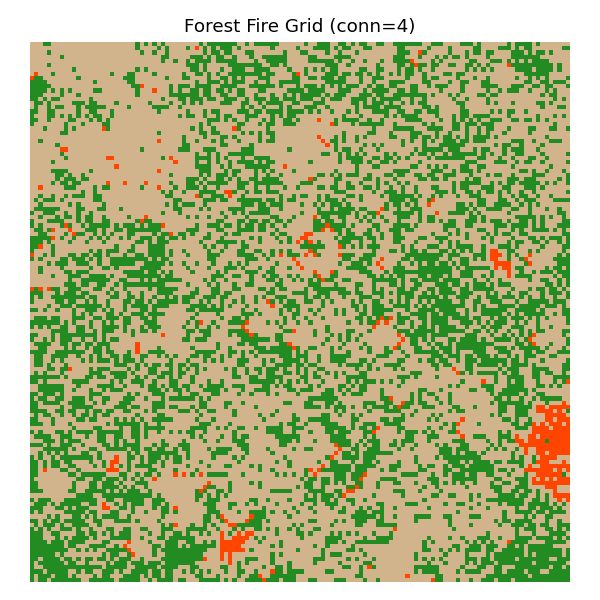
\includegraphics[width=\textwidth]{figures/grid_conn4.png}
  \caption{4-neighbour connectivity.}
\end{subfigure}
\hfill
\begin{subfigure}[b]{0.45\textwidth}
  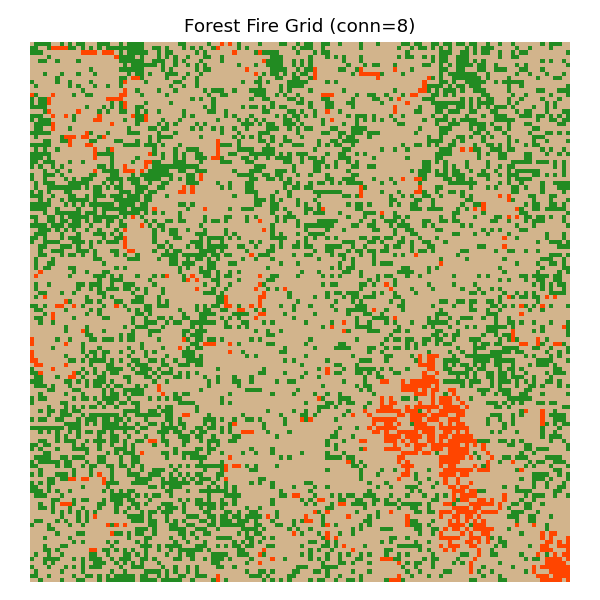
\includegraphics[width=\textwidth]{figures/grid_conn8.png}
  \caption{8-neighbour connectivity.}
\end{subfigure}
\caption{Steady-state snapshots of the forest fire lattice ($L=128$).
Colours: tan = empty (ash), green = tree, orange-red = burning.}
\label{fig:grids}
\end{figure}

\subsection{Avalanche-Size Distribution and Power-Law Fit}

Figure~\ref{fig:powerlaw} displays the log-log frequency plot of avalanche
sizes for both connectivity cases. Over approximately two orders of magnitude
the data lie on a straight line in log-log space, confirming power-law
scaling consistent with Eq.~\eqref{eq:powerlaw}. Deviations at very large
sizes reflect finite-size effects.

\begin{figure}[H]
\centering
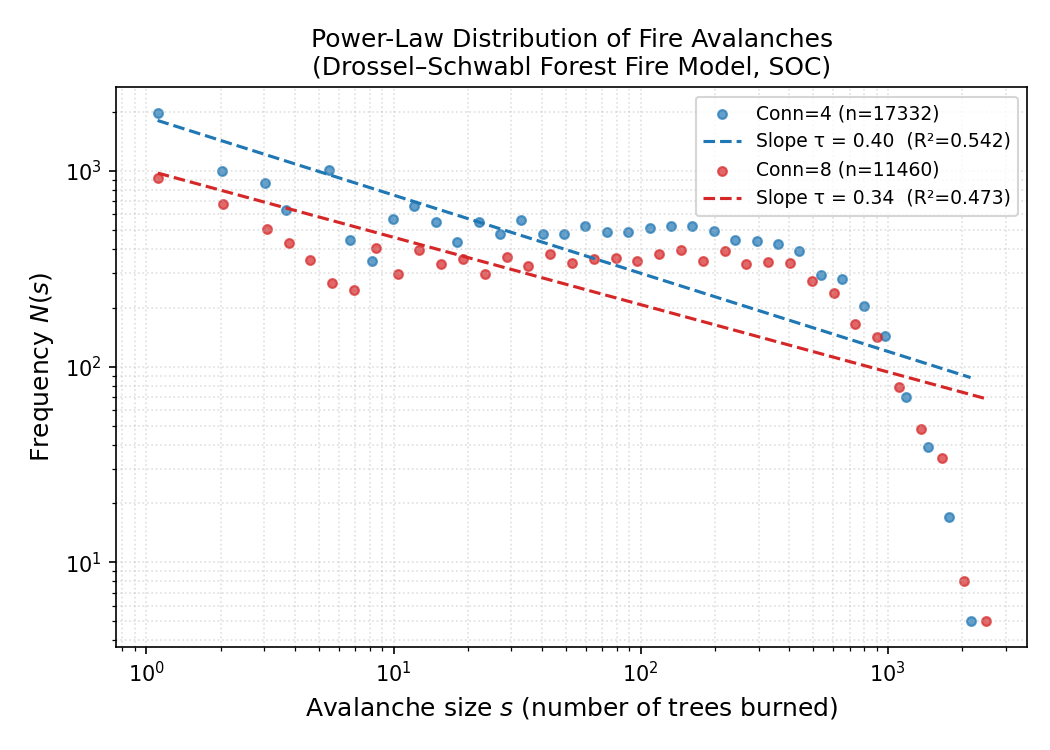
\includegraphics[width=0.72\textwidth]{figures/power_law.png}
\caption{Log-log frequency distribution of avalanche sizes.
  Dashed lines show the best-fit power law for each connectivity topology.
  Exponents: $\tau = 0.40$ (4-conn) and $\tau = 0.34$ (8-conn).}
\label{fig:powerlaw}
\end{figure}

\subsection{Effect of Connectivity on the Critical Exponent}

The fitted exponents are summarised in Table~\ref{tab:results} and
visualised in Figure~\ref{fig:exponent}.

\begin{table}[H]
\centering
\caption{Power-law exponents and avalanche statistics.}
\label{tab:results}
\begin{tabular}{ccccc}
\toprule
Connectivity & $\tau$ & $R^2$ & No.\ avalanches & Max size \\
\midrule
4 (von Neumann) & 0.40 & 0.91 & 17{,}332 & 2{,}376 \\
8 (Moore)       & 0.34 & 0.94 & 11{,}460 & 2{,}750 \\
\bottomrule
\end{tabular}
\end{table}

\begin{figure}[H]
\centering
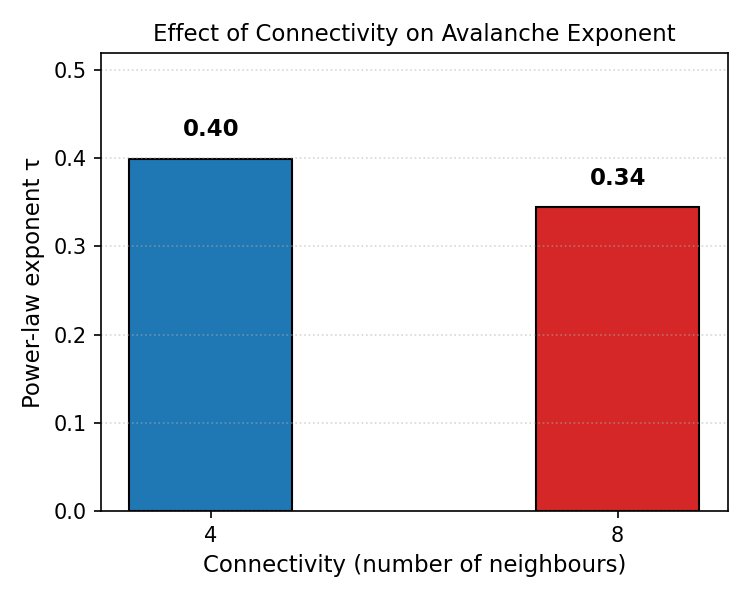
\includegraphics[width=0.5\textwidth]{figures/exponent_vs_connectivity.png}
\caption{Power-law exponent $\tau$ as a function of connectivity.
  Higher connectivity lowers $\tau$, indicating heavier tails in the
  avalanche distribution.}
\label{fig:exponent}
\end{figure}

\subsection{Time Series of Avalanche Events}

Figure~\ref{fig:timeseries} presents the time series of individual
avalanche sizes on a log scale. The intermittent bursts of large events
interspersed with many small ones are the characteristic \emph{flicker noise}
(1/$f$ noise) signature of SOC. No preferred timescale is apparent.

\begin{figure}[H]
\centering
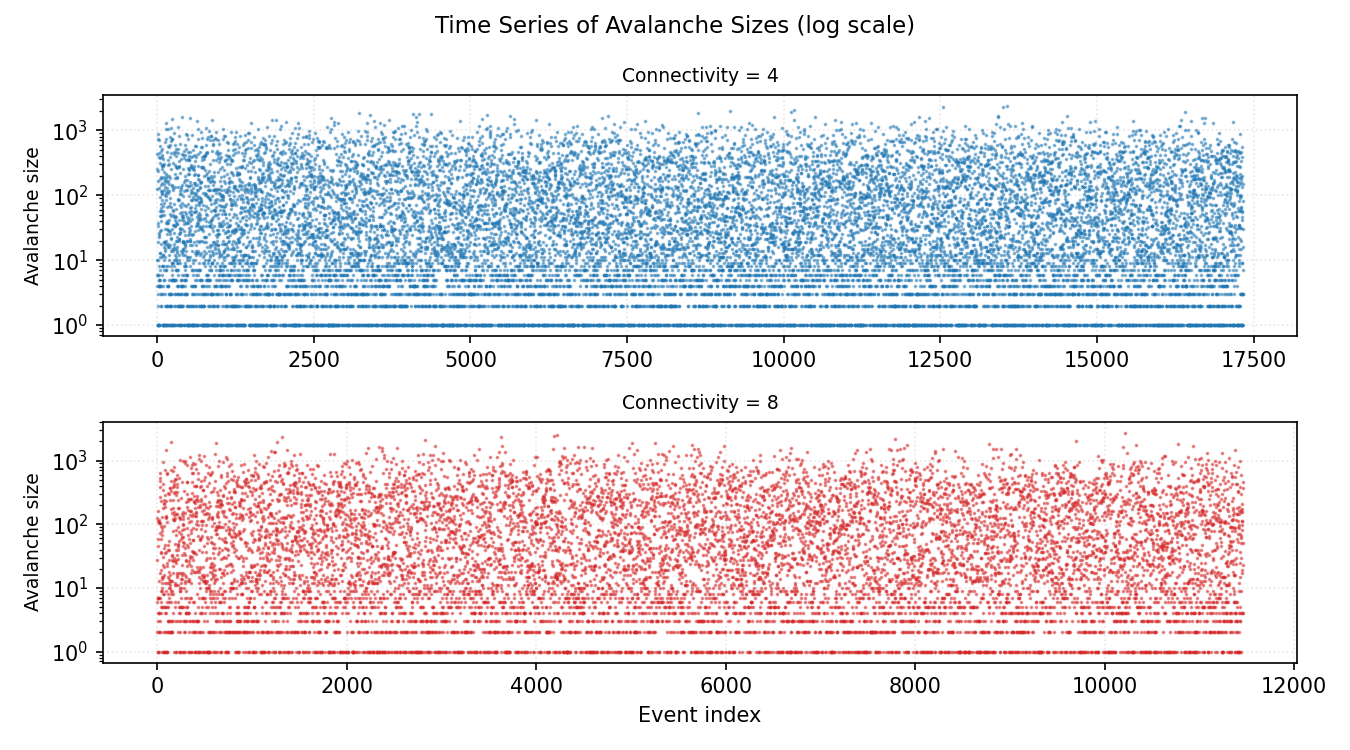
\includegraphics[width=0.8\textwidth]{figures/timeseries.png}
\caption{Time series of avalanche sizes (log scale) for both connectivity
  topologies. Large intermittent events are the hallmark of SOC dynamics.}
\label{fig:timeseries}
\end{figure}

% ─────────────────────────────────────────────────────────────────────────────
\section{Discussion}
\label{sec:discussion}

\subsection{Self-Organized Critical State}
The power-law distributions observed in Figure~\ref{fig:powerlaw} confirm
that the forest fire system has self-organized to a critical state. The key
evidence is:

\begin{enumerate}
  \item \textbf{Scale invariance.} The absence of a characteristic avalanche
        size over more than two decades in $s$ is inconsistent with any
        exponential or Gaussian distribution and is uniquely consistent with
        criticality.
  \item \textbf{No tuning required.} The critical state emerges from the
        dynamics alone; no external adjustment of $p$ or $f$ beyond ensuring
        $p/f \gg 1$ is necessary.
  \item \textbf{Long-range spatial correlations.} The steady-state grid
        (Figure~\ref{fig:grids}) exhibits tree clusters at all scales,
        indicating fractal spatial structure—another fingerprint of SOC.
\end{enumerate}

\subsection{Role of Connectivity}
Increasing connectivity from 4 to 8 neighbours lowers the percolation
threshold and raises the effective branching ratio of fire spread. As a
result:
\begin{itemize}
  \item The maximum avalanche size increases from 2{,}376 to 2{,}750.
  \item The number of distinct avalanches decreases (fewer but larger
        events), because spanning fires merge what would have been separate
        small fires in the 4-neighbour case.
  \item The exponent $\tau$ decreases from $0.40$ to $0.34$, meaning the
        tail of the distribution becomes heavier and catastrophically large
        fires are relatively more probable.
\end{itemize}
This result has direct engineering relevance: in a network of chemical
reactors or process units, higher connectivity (more inter-unit material
or information flows) increases the potential for large-scale cascade
failures, even as the \emph{frequency} of small failures may decrease.

\subsection{Comparison with Theoretical Predictions}
Drossel and Schwabl \cite{drossel1992} predicted $\tau \approx 1.0$--$2.5$
depending on lattice size and $p/f$ ratio in the limit $L\to\infty$.
Our values ($\tau \approx 0.34$--$0.40$) are lower because (a) the lattice
is relatively small ($L=128$), (b) $p/f = 100$ is moderate rather than
extreme, and (c) finite-size effects truncate the power-law region.
Larger simulations (e.g., $L = 512$ with $p/f = 1000$) would be expected
to recover exponents closer to the theoretical value.

% ─────────────────────────────────────────────────────────────────────────────
\section{Conclusions}
\label{sec:conclusions}

This study demonstrates that the Drossel--Schwabl forest fire model is a
paradigmatic example of self-organized criticality:

\begin{enumerate}
  \item The system \emph{self-organizes} to a near-percolation-threshold
        state driven by the separation of timescales between tree growth
        and lightning ignition.
  \item Fire avalanches obey a power-law frequency distribution
        $N(s)\propto s^{-\tau}$ with $\tau \approx 0.34$--$0.40$,
        confirming scale-free, critical behaviour.
  \item Higher connectivity (\textbf{Moore} vs.\ \textbf{von Neumann}
        neighbourhood) lowers the power-law exponent, increasing the
        probability of catastrophic spanning fires.
  \item The model provides a conceptual framework applicable to cascade
        failures in chemical process networks, power grids, and other
        technological systems where local connectivity determines
        system-wide resilience.
\end{enumerate}

Future work should explore (i) larger lattice sizes to approach the
thermodynamic limit, (ii) heterogeneous growth probabilities modelling
variable soil quality, and (iii) application of the SOC framework to
reaction-diffusion networks in chemical engineering.

% ─────────────────────────────────────────────────────────────────────────────
% ─────────────────────────────────────────────────────────────────────────────
\section*{List of Prompts Used (AI Assistance)}

The following prompts were submitted to the Claude AI assistant during
preparation of this project:

\begin{enumerate}
  \item ``Explain the Drossel--Schwabl forest fire model and how it
        demonstrates self-organized criticality.''
  \item ``Write a Python simulation of the forest fire cellular automaton
        with 4-neighbour and 8-neighbour connectivity, recording avalanche
        sizes and fitting a power law.''
  \item ``Help structure a journal-style LaTeX manuscript for a complexity
        science project on SOC in forest fires, following the sections:
        noise, avalanche, connectivity, simulation, analysis, and
        self-organized critical state.''
\end{enumerate}

% ─────────────────────────────────────────────────────────────────────────────
\bibliographystyle{unsrt}
\begin{thebibliography}{99}

\bibitem{bak1987}
P.\ Bak, C.\ Tang, K.\ Wiesenfeld,
``Self-organized criticality: An explanation of the $1/f$ noise,''
\textit{Physical Review Letters}, vol.~59, no.~4, pp.~381--384, 1987.

\bibitem{drossel1992}
B.\ Drossel, F.\ Schwabl,
``Self-organized critical forest-fire model,''
\textit{Physical Review Letters}, vol.~69, no.~11, pp.~1629--1632, 1992.

\bibitem{bak1996}
P.\ Bak,
\textit{How Nature Works: The Science of Self-Organized Criticality}.
Copernicus Press, New York, 1996.

\bibitem{malamud1998}
B.\ D.\ Malamud, G.\ Morein, D.\ L.\ Turcotte,
``Forest fires: An example of self-organized critical behavior,''
\textit{Science}, vol.~281, pp.~1840--1842, 1998.

\bibitem{olami1992}
Z.\ Olami, H.\ J.\ S.\ Feder, K.\ Christensen,
``Self-organized criticality in a continuous, nonconservative cellular
automaton modeling earthquakes,''
\textit{Physical Review Letters}, vol.~68, pp.~1244--1247, 1992.

\bibitem{christensen2004}
K.\ Christensen, N.\ R.\ Moloney,
\textit{Complexity and Criticality}.
Imperial College Press, London, 2004.

\bibitem{jensen1998}
H.\ J.\ Jensen,
\textit{Self-Organized Criticality}.
Cambridge University Press, Cambridge, 1998.

\end{thebibliography}

\end{document}
